\documentclass{sigchi}

% Use this section to set the ACM copyright statement (e.g. for
% preprints).  Consult the conference website for the camera-ready
% copyright statement.

% Copyright
%\CopyrightYear{2020}
%\setcopyright{acmcopyright}
%\setcopyright{acmlicensed}
%\setcopyright{rightsretained}
%\setcopyright{usgov}
%\setcopyright{usgovmixed}
%\setcopyright{cagov}
%\setcopyright{cagovmixed}
% DOI
%\doi{https://doi.org/10.1145/3313831.XXXXXXX}
% ISBN
% \isbn{978-1-4503-6708-0/20/04}
%Conference
\conferenceinfo{CHI'20,}{April  25--30, 2020, Honolulu, HI, USA}
%Price

% Use this command to override the default ACM copyright statement
% (e.g. for preprints).  Consult the conference website for the
% camera-ready copyright statement.

%% HOW TO OVERRIDE THE DEFAULT COPYRIGHT STRIP --
%% Please note you need to make sure the copy for your specific
%% license is used here!
% \toappear{
% Permission to make digital or hard copies of all or part of this work
% for personal or classroom use is granted without fee provided that
% copies are not made or distributed for profit or commercial advantage
% and that copies bear this notice and the full citation on the first
% page. Copyrights for components of this work owned by others than ACM
% must be honored. Abstracting with credit is permitted. To copy
% otherwise, or republish, to post on servers or to redistribute to
% lists, requires prior specific permission and/or a fee. Request
% permissions from \href{mailto:Permissions@acm.org}{Permissions@acm.org}. \\
% \emph{CHI '16},  May 07--12, 2016, San Jose, CA, USA \\
% ACM xxx-x-xxxx-xxxx-x/xx/xx\ldots \$15.00 \\
% DOI: \url{http://dx.doi.org/xx.xxxx/xxxxxxx.xxxxxxx}
% }

% Arabic page numbers for submission.  Remove this line to eliminate
% page numbers for the camera ready copy
% \pagenumbering{arabic}

% Load basic packages
\usepackage{balance}       % to better equalize the last page
\usepackage{graphics}      % for EPS, load graphicx instead 
\usepackage[T1]{fontenc}   % for umlauts and other diaeresis
\usepackage{txfonts}
\usepackage{mathptmx}
\usepackage[pdflang={en-US},pdftex]{hyperref}
\usepackage{color}
\usepackage{booktabs}
\usepackage{textcomp}


% Some optional stuff you might like/need.
\usepackage{microtype}        % Improved Tracking and Kerning
% \usepackage[all]{hypcap}    % Fixes bug in hyperref caption linking
\usepackage{ccicons}          % Cite your images correctly!
% \usepackage[utf8]{inputenc} % for a UTF8 editor only

% If you want to use todo notes, marginpars etc. during creation of
% your draft document, you have to enable the "chi_draft" option for
% the document class. To do this, change the very first line to:
% "\documentclass[chi_draft]{sigchi}". You can then place todo notes
% by using the "\todo{...}"  command. Make sure to disable the draft
% option again before submitting your final document.
\usepackage{todonotes}

% Paper metadata (use plain text, for PDF inclusion and later
% re-using, if desired).  Use \emtpyauthor when submitting for review
% so you remain anonymous.
\def\plaintitle{The Far Journey}
\def\plainauthor{First Author, Second Author, Third Author,
  Fourth Author, Fifth Author, Sixth Author}
\def\emptyauthor{}
\def\plainkeywords{Authors' choice; of terms; separated; by
  semicolons; include commas, within terms only; this section is required.}
\def\plaingeneralterms{Documentation, Standardization}

% llt: Define a global style for URLs, rather that the default one
\makeatletter
\def\url@leostyle{%
  \@ifundefined{selectfont}{
    \def\UrlFont{\sf}
  }{
    \def\UrlFont{\small\bf\ttfamily}
  }}
\makeatother
\urlstyle{leo}

% To make various LaTeX processors do the right thing with page size.
\def\pprw{8.5in}
\def\pprh{11in}
\special{papersize=\pprw,\pprh}
\setlength{\paperwidth}{\pprw}
\setlength{\paperheight}{\pprh}
\setlength{\pdfpagewidth}{\pprw}
\setlength{\pdfpageheight}{\pprh}

% Make sure hyperref comes last of your loaded packages, to give it a
% fighting chance of not being over-written, since its job is to
% redefine many LaTeX commands.
\definecolor{linkColor}{RGB}{6,125,233}
\hypersetup{%
  pdftitle={\plaintitle},
% Use \plainauthor for final version.
%  pdfauthor={\plainauthor},
  pdfauthor={\emptyauthor},
  pdfkeywords={\plainkeywords},
  pdfdisplaydoctitle=true, % For Accessibility
  bookmarksnumbered,
  pdfstartview={FitH},
  colorlinks,
  citecolor=black,
  filecolor=black,
  linkcolor=black,
  urlcolor=linkColor,
  breaklinks=true,
  hypertexnames=false
}

% create a shortcut to typeset table headings
% \newcommand\tabhead[1]{\small\textbf{#1}}

% End of preamble. Here it comes the document.
\begin{document}

\title{\plaintitle}

\numberofauthors{2}
\author{%
  \alignauthor{James Blankenship\\
    \affaddr{for Submission}\\
    \affaddr{Crockett Mills, US}\\
    \email{jamcblan@ut.utm.edu}}\\
  \alignauthor{Andrew Marshall\\
    \affaddr{for Submission}\\
    \affaddr{Martin, US}\\
    \email{jesamars@ut.utm.edu}}\\
  }

\maketitle

\begin{abstract}
 Our project is a 3D real time game in the Unreal engine. 
  The game is a fantasy genre in a medieval setting. The game will have 3 levels in it.
  It will have a variety of enemies and weapons. There will be magic. The different types of magic for the player to use would include pyromancy and sorcery.There will be a class system that has two classes.The two classes are the Mage and the Warrior. Each level will have a boss enemy in it.
   \end{abstract}



\section{Introduction}
To introduce this project, we decided to develop a game, and the game will have the title of "The Deep Journey." This game is in the first person. The general setting is that of medieval fantasy, and it will have 3 different levels The first level will be where the character will start out in, and it will be the castle level. The castle includes two courtyards and a middle building. The second level will be the castles dungeon which will have holding cells for enemies and middle room where the main boss is. The third level will be the fort area which will be a walled structure with small buildings. The main building for the level will be a tavern which will hold the boss. The character player will have a different type of weapons to choose from which will include hammer or staffs. The character player will face off against different enemies types, including orcs, and wolves.The character will also be able to wield different magic. There will be two different magic the character can wield: pyromancy and sorcery. 

\section{Motivations}
Motivations for making a game is that James and Andrew play video games. Also, it was the easiest to grasp the concept of how to build the game compared to the other options we came up with. We chose the fantasy setting because of something we saw in another class. We chose the enemy type because James likes orcs. Also, in many types of media, they are seen as the bad guys. An example of this is the orcs from The Lord of the Rings. We chose first person combat game aspect since having a live combat compared to turn based is more interesting to us.Unreal was the main choice since, after research online, it showed that Unreal was the easier of the two compared to Unity.
\section{Technical specifications}
We are using Unreal Engine for our project. We use blueprints in Unreal for most things and behavior trees for the AI. Behavior trees are essentially used to create AI by having branches that determine actions. We will use blueprints in places that require simple execution, such as taking the player to a new level. An example would be the AI just searching, and then it will execute a different branch when it finds someone. GitHub is being used for collaboration with each other and version control. All the assets that are currently being used are in the Unreal Store.
\section{Levels}
There are three levels in this game. The first is the castle area, and it was the first one made. It is divided into two courtyards and a main building; each courtyard will have some smaller enemies for you to deal with. The middle building will have two stories. The first one is just a way to get to the other courtyard, basement level, and upstairs. The second level will hold the boss enemy for the level. The second level is the basement/dungeon. It is a smaller level with just two holding cells and a backroom for the boss and some enemies. The third level is a bigger level with a bunch of small buildings in an enclosed space. It has wolves and orcs next to the building, with a tavern in the back with the boss.
\subsection{Castle}
We chose a castle for the first level because we wanted to remind the player that they are playing a fantasy game. It is also very simple concept-wise, since a castle is basically a big building with courtyards. The castle level was the first, so it required the most research on how to make it look at least decent. The ground section of the floor is made using a special tool in landscape mode that makes a big smooth surface on the floor. After that, we added small bumps in the ground to give it a realistic texture since having a flat texture surface would look a little boring. Since it was the first level, it still has some roughness around the edges, such as some parts of the building not being connected exactly to each other, but we were able to move walls around to make it look presentable. The enemy choice for this level is simple since it is the first level and did not want to overwhelm the player with enemies in the level. The level has very few enemies in total, and they are spread out. The boss was also there by itself in the middle building to make the level easy. The only thing difficult about the level is the boss and that the player is immediately thrown into combat at the start of the game. 
\begin{figure}


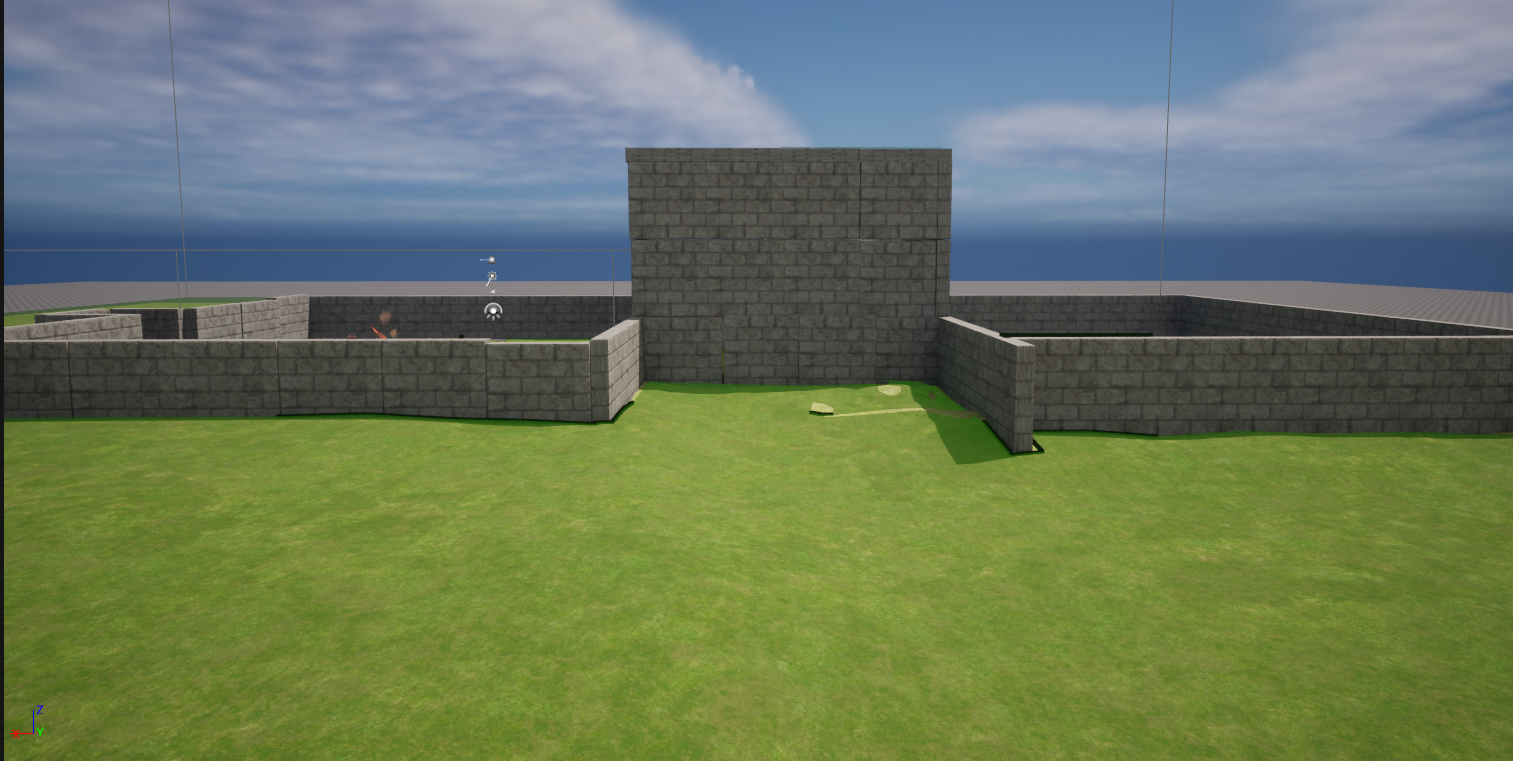
\includegraphics[width=6.5cm, height=6.5cm]{Figure/castle.png}
\caption{Castle level}
\end{figure}
\subsection{Basement}
The basement level was chosen because it would make sense for a castle to have a basement/dungeon area that contains prisoners and other enemies. This also helped make the transitions between the castle and basement more natural. For the basement level, the player character was supposed to feel uneasy. This feeling of unease was accomplished by having the lighting be recessed and letting the shadows, combined with a lack of sunlight, create a dark and scary atmosphere. The level also contains a couple of cells that house different prisoners from the castle. The layout of the level consists of a long corridor with two different hallways on the left and right. One of the npcs that the character can see housed in the cells is a giant chicken that incorporates custom animation work that we designed and implemented. The main corridor contains a large room that houses many enemies that all rush the player's character. The character player was meant to be caught off guard by the great number of enemies, adding to the difficulty of the level..
\begin{figure}


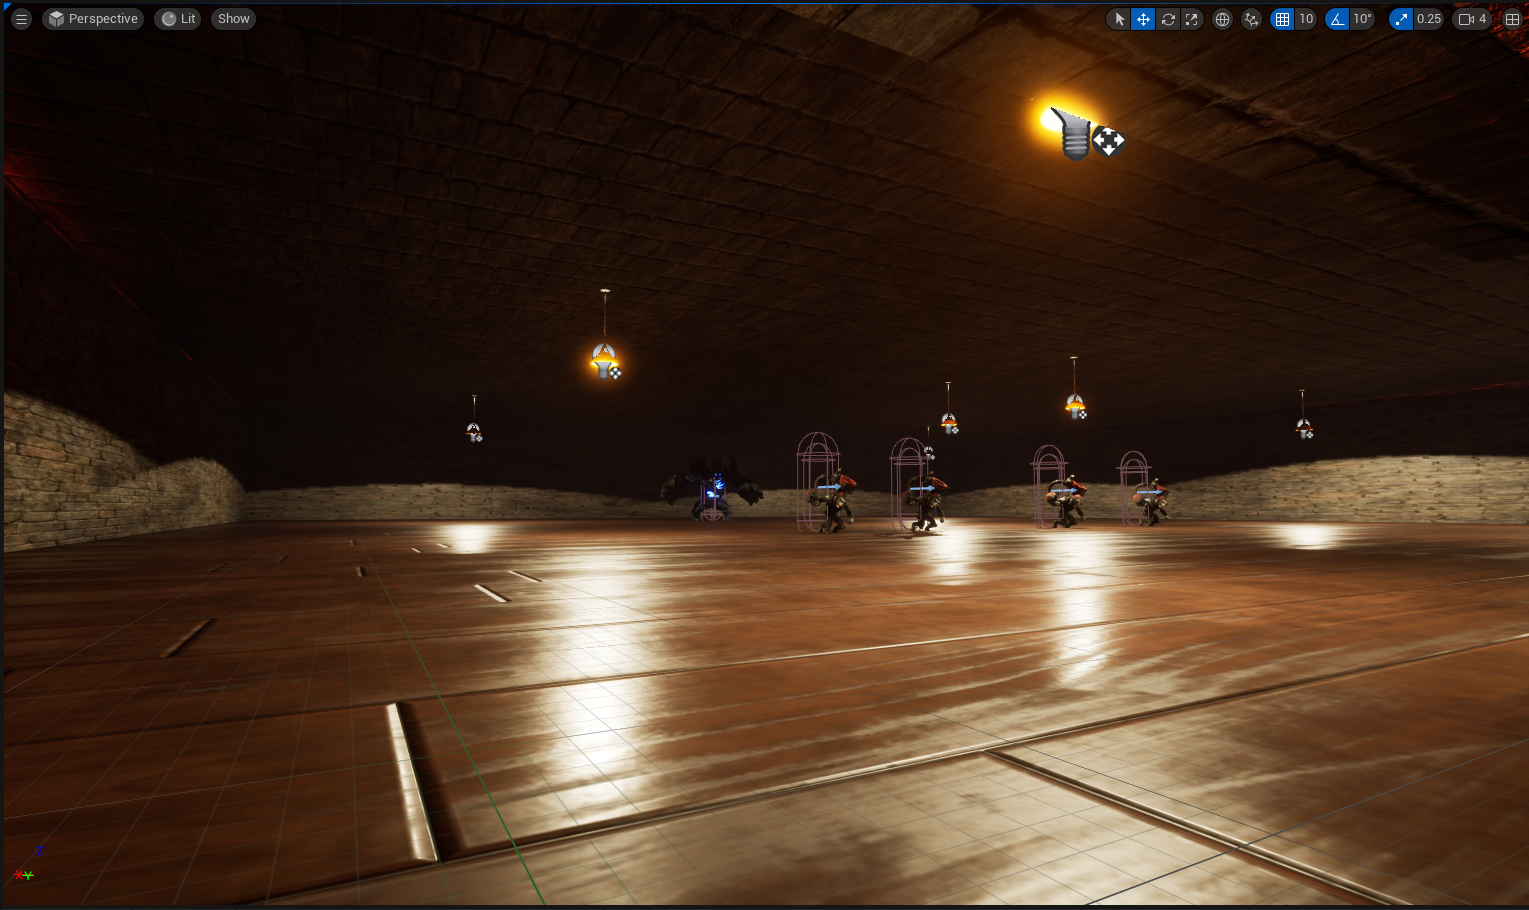
\includegraphics[width=6.5cm, height=6.5cm]{Figure/basement.png}
\caption{Basement Level}
\end{figure}
\subsection{Fort}
The third and final level was one of the easier levels to make since we were getting better at level building. In Unreal, you can highlight multiple objects and copy them. That was how the walls for the castle were made. Something similar was done with small buildings, but it was done with the whole building. The floor of this level was simple to construct because we had already done so in the castle level. The enemies at this level are simple compared to those at other levels since they stand there, and guard the buildings. The enemies are more difficult since there are multiple groups of them. The boss is also accompanied by two wolves, making the tavern battle more difficult. I chose the fort as a level since I wanted an area that would mainly focus on the orcs, and an area in the woods made the most sense to me.
\begin{figure}


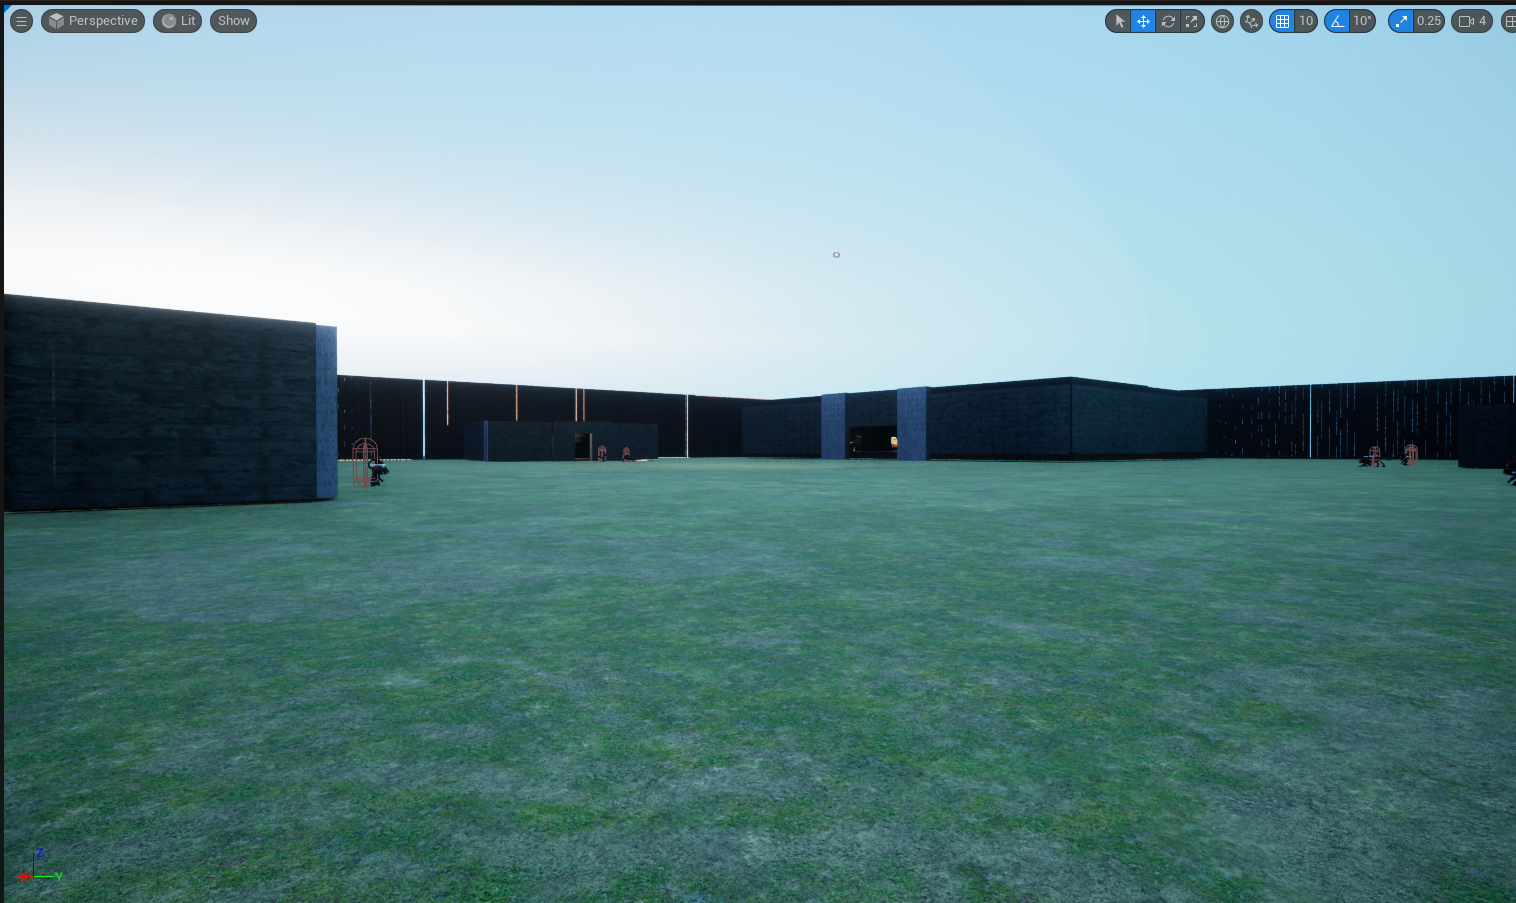
\includegraphics[width=6cm, height=6cm]{Figure/fort.png}  
\caption{Fort level}
\end{figure}
\section{Classes}
We made two classes for the game: the mage and the warrior. The warrior was the first class made and is the simpler of the two. Its first ability is just a healing ability, which is useful for staying alive since you have to be in melee combat. The second ability is a damage buff, which will give double damage to his attacks. The third ability is his ultimate, which gives health regeneration to the player. The mage class is the DPS class. The first ability sends out fast-moving disks in front of the player. The second ability shoots a fireball, which does a lot of damage, which is useful for the bosses in the game. The ult will regenerate the players' resources so they can cast more spells.

 
\begin{figure}


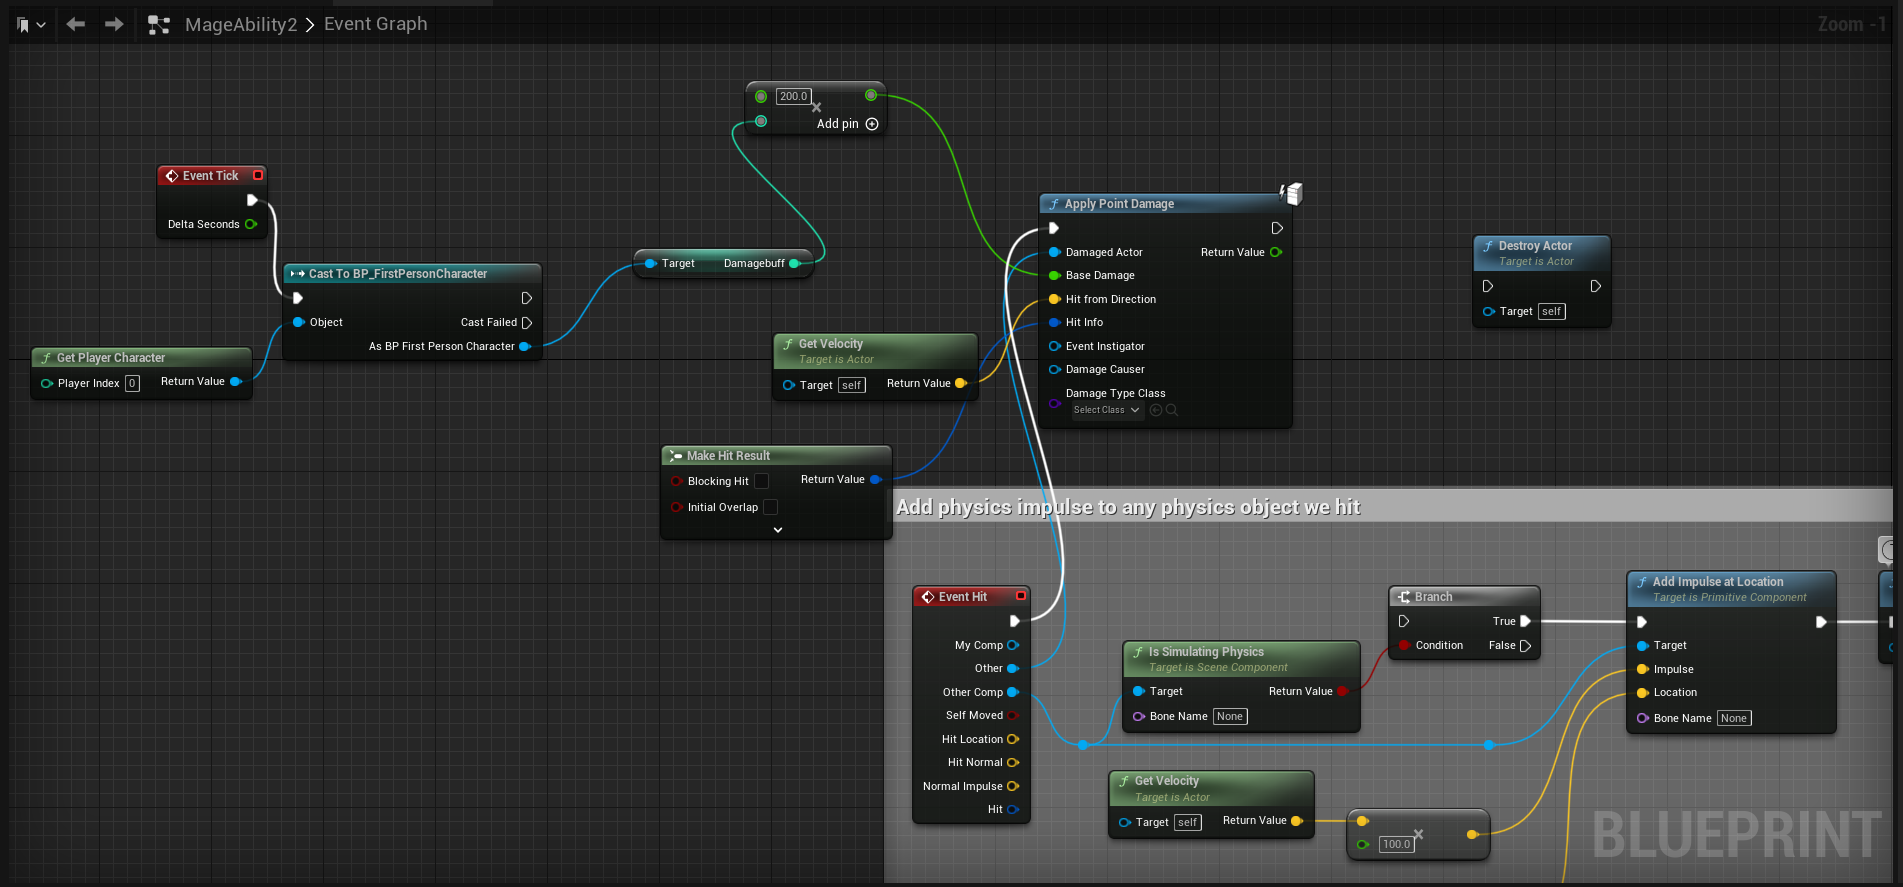
\includegraphics[width=6cm, height=6cm]{Figure/MageAbility.png}
\caption{Mage blueprint}
\end{figure}

\section{What we learned}
This section will cover what we learned over the course of making our project. Over the semester, we learned about game development within Unreal Engine 5. Unreal Engine is made by Epic Games and is free to use. We also learned how to go about making a game and all the steps that require it. Making the game involved many things, like having to plan out the different levels within the game, choosing an overall art direction for the game, deciding on what enemies the player will go up against, and deciding on the different abilities the player character will have. Something else we learned how to do was create custom animations within the Unreal Engine. The enemies and the AI that is used to make them work were something else we learned. The player characters' different projectiles and weapons that can be used were implemented. An interface for the player's character that shows the player's health, magic, and ultimate ability was made.
\section{blueprints}
The major blueprints that were made dealt with classes. The projectiles used were modified blueprints of the original projectile. The damage and speed numbers for gravity and speed were changed. To achieve the effect of healing, the warrior class systems used the changing of simple variable values. We had similar effects on other values, such as resources and ultimate bars. We achieved the damage buff ability by having a damage buff variable, having it change from 1 to 2, and having it affect weapon damage. Each weapon that benefits from the effect needed to have the variable added to it and changed by the variable. The only problem I had with that was the casting of the player character, which required finding more information about casting online. All casting in Unreal allows you to work with information from another blueprint, which is useful when dealing with abilities. The mage abilities used similar blueprints since it was just spawning the projectile, and the only thing that was different was the damage numbers and the cost of using the ability. To regenerate that bar, the ultimates simply had a timer run over a different variable. Choosing your class added some complexity to the blueprints since you had to have conditionals for the abilities. It was done by adding a variable to keep track of what class you have. The class choice system is done by clicking a key on the keyboard and choosing what weapon you want to use. The weapon choice system just binds the weapon to your skeleton. The weapon is not conjured into the game; it already exists in the level, and it just moves it to you.
\begin{figure}
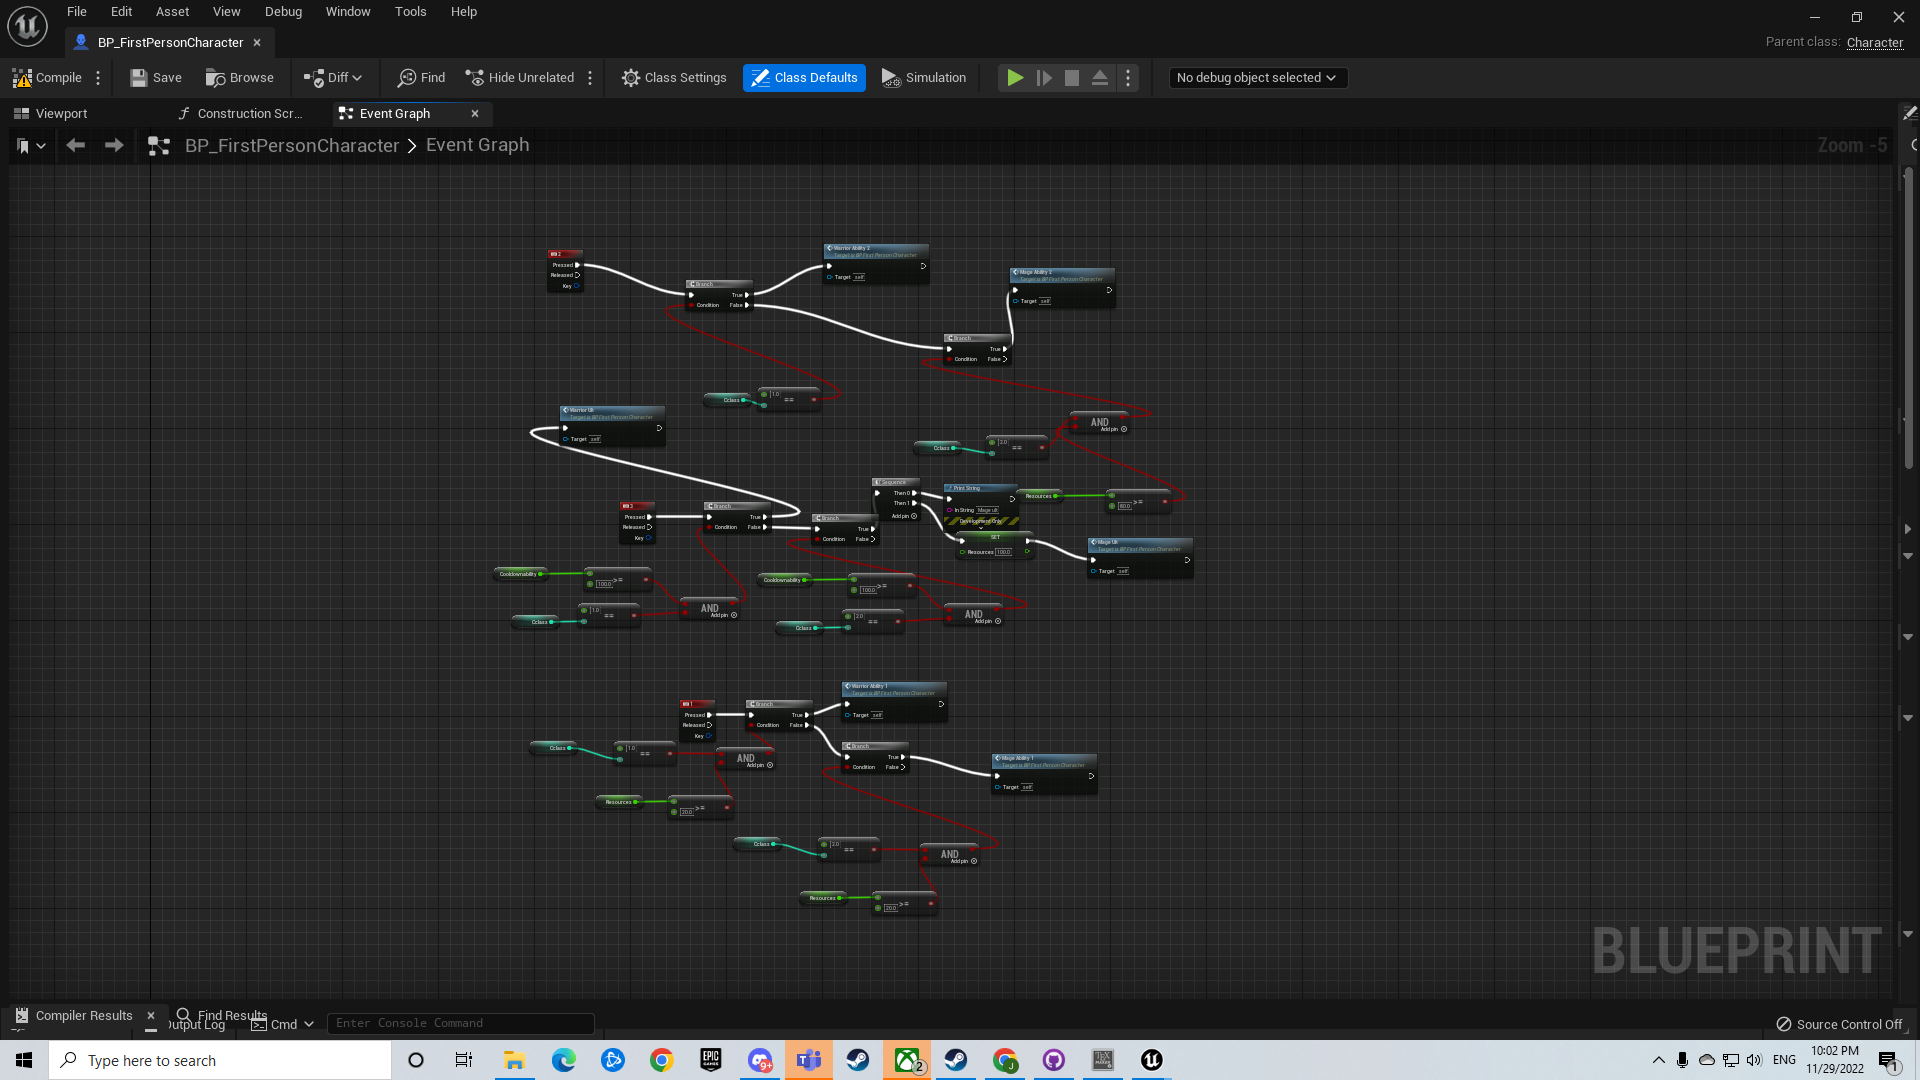
\includegraphics[width=6.5cm, height=6.5cm]{Figure/blueprint.png}
\caption{Example Blueprint}
\end{figure}
\subsection{AI}
AI was a little tricky since at first I just had simple blueprints to do basic tasks such as see and move towards the player. That later changed when I learned about behavior trees. All a behavior tree does is choose paths and execute commands. A common command is the turn enemy command, which causes the enemy to turn to face the player. The movement is basically the AI finding a spot nearby and moving towards it until it sees the player. The AI will make the enemy move towards the player. This part of the project was difficult, and we had to use a tutorial made by Unreal to get more information about behavior trees and get basic functionality.
\begin{figure}


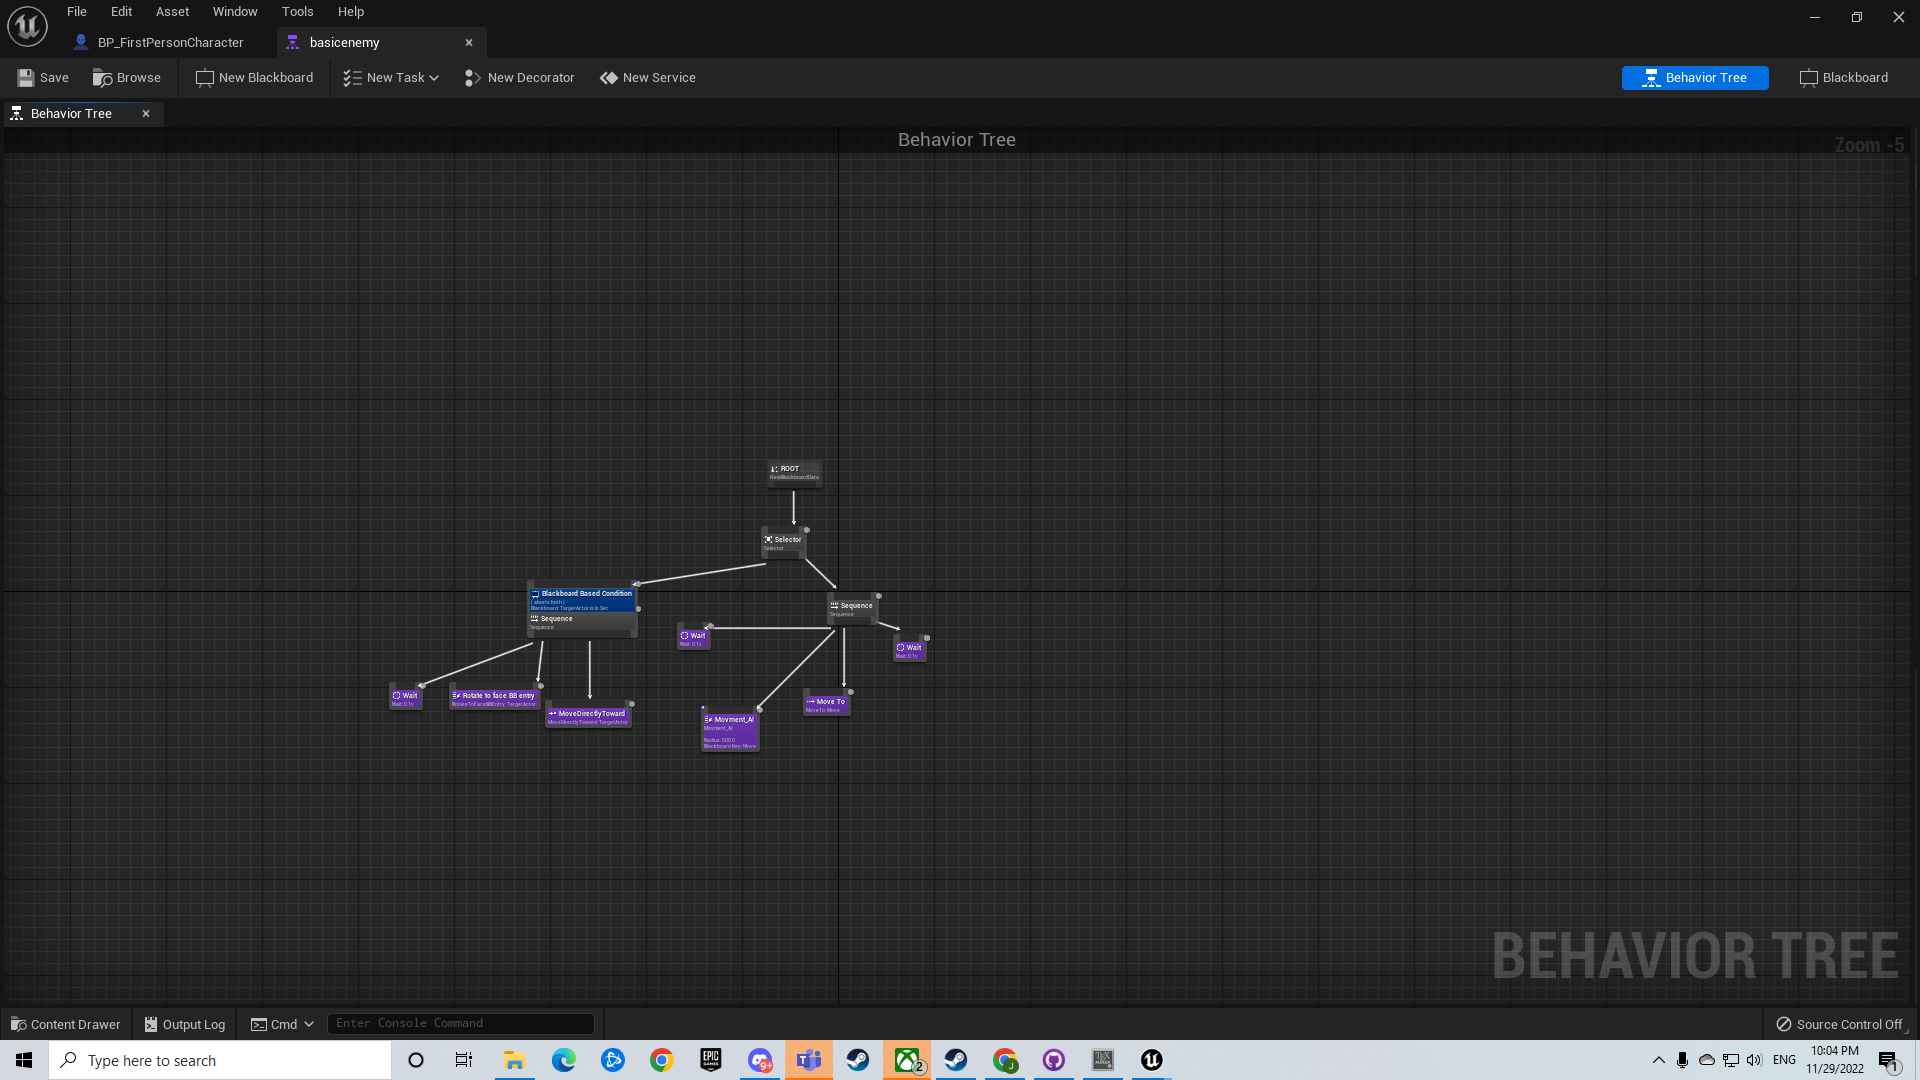
\includegraphics[width=6.5cm, height=6.5cm]{Figure/AI.png}  
\caption{AI}
\end{figure}
\section{Trials and Tribulations}
While creating and perfecting the project, we encountered certain issues. Even though we used GitHub for our version control and collaboration, we still ran into problems where we lost work. The most notable was the addition of animations to the melee weapon and later. Some projectiles stopped working, and the melee animation stopped working. The main fix for that was that, towards the end, James was the only one allowed to push to the master branch. Another issue encountered was the differences in performance, specifically GPU power, between our personal machines, which complicated development. The fix was that James was the one who did most of the live testing, since trying at 5 fps was a bad idea. Also, the lighting was weird depending on whose computer we were using. On one computer, it looked fine, but on another, the lighting seemed off. That never got fixed in the final project since we focused on mechanics, and it got put on the backlog. Some concepts were difficult, such as the AI. The AI had trouble when dealing with different levels and would lead to different actions or inactions being made by the AI, most noticeable being the guard AI in the second and third levels. There are also a lot of options on the blueprints and objects, so it was easy to get overwhelmed by them. Implementing the classes was tedious since choosing a class and a weapon cannot be on the same keybinds. The class ultimate was difficult since loops are awful in the blueprint system, and would throw a no end condition error. We had to use timers, which are much easier to deal with in blueprints.

\section{Future Work}
There are some areas in our project that we weren't able to implement and could be considered future work. The first idea we had was porting the game to mobile. This is possible because unreal engines work cross platform. More levels being added was something else we would like to do in the future. Adding more enemies and weapons to the player character is something we could work on later down the road. 


\section{Project Development}
The project started with just a map that later became the empty castle. At first, it was just messing with the toolkit to figure things out. For example, the floor is made from Unreal's toolkit instead of just adding floor blocks. The textures on the walls needed to look good. The easy solution for that was just repeating a wall block, which was good for our use. I later added enemies that just stood there, and then later they would move randomly. We started working on the second level, which became the basement level, since it seemed to transition well. The level transitions were done using trigger boxes, which are boxes that, when stepped over, will execute code. We did this for all the level transitions and when the player died. The levels after the castle stayed stagnant since we focused on the mechanics of the game. It first started with the AI, which was a nightmare to work with, so we switched over to working on the class system since it was easier. We added a warrior class with abilities such as healing, damage buffs, and a regeneration ability. The ultimates required us learning about timers since they were required to make it work. The mage was the next class made, and it had different spells it could use. The spells required us to make more projectiles with different stats. We then shifted focus back to the AI and got them to move around.


\section{Opinions on Project}
The project was overall helpful for learning about different software, and it forced us to look for information online for help. Example: the AI was difficult since it required multiple blueprints and a blackboard. It also required making an AI controller for the enemies to use. We would have never figured that out unless we looked online for help. We also need to look up tutorials for the AI and the UI. Unreal does not really show you how to do things on its service.


\section{Conclusion}
To conclude over the semester with our project, we were able to make a playable first person action game. This game was called the deep journey, and we developed it using unreal engine 5. We used the blueprint system within unreal engine 5 to deal with the different player classes, and connect the levels using trigger boxes. The project development started out with just one level, and by the end we had three distinct levels with different enemies the players could fight using their classes abilities. The project helped us learn game development and the new toolkits we needed to use. We have improvements and additions to the project that could be completed in the future. Overall, this project was a fun way to show our resourcefulness/work ethic as computer science majors, and showcase how we can use the knowledge we've procured over the years to accomplish great things.




% Balancing columns in a ref list is a bit of a pain because you
% either use a hack like flushend or balance, or manually insert
% a column break.  http://www.tex.ac.uk/cgi-bin/texfaq2html?label=balance
% multicols doesn't work because we're already in two-column mode,
% and flushend isn't awesome, so I choose balance.  See this
% for more info: http://cs.brown.edu/system/software/latex/doc/balance.pdf
%
% Note that in a perfect world balance wants to be in the first
% column of the last page.
%
% If balance doesn't work for you, you can remove that and
% hard-code a column break into the bbl file right before you
% submit:
%
% http://stackoverflow.com/questions/2149854/how-to-manually-equalize-columns-
% in-an-ieee-paper-if-using-bibtex
%
% Or, just remove \balance and give up on balancing the last page.
%
\balance{}




\cite{unrealweb}. \cite{wizard} \cite{infinityw} \cite{infinitya} \cite{AI}  \cite{Timer} \cite{health}


% BALANCE COLUMNS
\balance{}

% REFERENCES FORMAT
% References must be the same font size as other body text.
%%\bibliographystyle{SIGCHI-Reference-Format}
%% \bibliographystyle{acm-sigchi-proceedings}

\bibliographystyle{plain}
\bibliography{bibliography}

\end{document}


